% SPDX-License-Identifier: LPPL-1.3c
% Copyright (C) 2026 Christophe Jorssen
% Author and Current Maintainer: Christophe Jorssen <christophe.jorssen@gmail.com>
% LPPL maintenance status: maintained
% This file is part of luafemm. See LICENSE and LICENSES.md for its terms.
\section{Regional measurements, forces and torques}
\label{sec:postprocessing}
This chapter describes planar measurements. Axisymmetric volume weights,
component names and force restrictions are specified in Section~\ref{sec:axisymmetric}.
The planar postprocessor works on the same unsmoothed, piecewise-constant field that
produces the field lines. A \emph{selection} identifies existing elements;
a \emph{measurement} solves if necessary and records a named numerical snapshot.
The snapshot can be printed, plotted or drawn as a force arrow. There is no
external process, temporary data table or shell escape.

\subsection{From a drawing to a measured attraction}
Declare all physical regions and set a positive problem |depth| first. Then
select the moving body, request its force and draw the result. For example,
after constructing the U electromagnet used below:
\begin{codeexample}[code only]
\path[femm/selection={name=armature,material=armco-pure-iron}]
  (-42,31) rectangle (42,55);
\path[femm/measure={name=pull,selection=armature,quantity=force}];
\pic[femm/force={result=pull}] {femm force};
\end{codeexample}
The selection rectangle is not another material region. It restricts the
|armco-pure-iron| filter to the armature, leaving the core out. The default force
method automatically constructs a weighting field through the surrounding air.
Its orange arrow starts at the selected area's centroid, has an illustrative
length of 12 model units and carries a label in newtons.

The complete example varies both gaps together, retains the three results and
plots the attraction. Start with these draft settings, then reduce mesh size
and gap spacing targets and compare the \emph{force}, not just the appearance
of the field lines. Increasing the number of plotted field lines does not
improve the mechanical result.
\luafemmexamplebegin{forces}

% manual example: forces/1

\begin{codeexample}[setup code]
\pgfkeys{/femm/measure/pull/.style={
  quantity=force,selection=armature,method=weighted}}
\tikzset{femm force arrow/.append style={red!75!black}}
\end{codeexample}

The following picture uses the preceding definitions.

% manual example: forces/2

\begin{codeexample}[width=5.2cm]
\foreach \gap/\result in {2/gap-two,4/gap-four,6/gap-six}{
  \begin{tikzpicture}[scale=.48,femm/problem={
    xmin=-70,xmax=70,ymin=-60,ymax=75,
    mesh size=5,depth=10}]
    \node[femm/u electromagnet={
      width=80,height=60,leg thickness=15,
      gap=\gap,armature thickness=15,
      ampere turns=2000,gap mesh size=1,
      core material=armco-pure-iron,armature material=armco-pure-iron},
      anchor=core center] (M) {};

    \path[femm/selection={name=armature,material=armco-pure-iron}]
      (-42,31) rectangle (42,55);
    \path[femm/measure={pull,name=\result,parameter=\gap}];
    \begin{scope}
      \clip (-53,-37) rectangle (53,65);
      \pic[femm/lines=13] {femm field};
    \end{scope}
    \pic[femm/force={result=\result,length=16}] {femm force};
    \node[font=\small] at (0,-43) {Gap: $\gap\,\mathrm{mm}$};
  \end{tikzpicture}
}
\end{codeexample}

% manual example: forces/3

\begin{codeexample}[width=5.2cm]
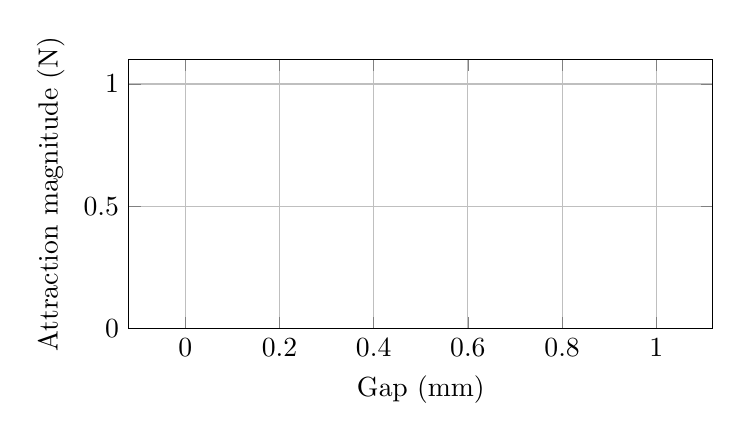
\begin{tikzpicture}
  \begin{axis}[width=9cm,height=5cm,grid=major,
    xlabel={Gap (mm)},ylabel={Attraction magnitude (N)},
    ymin=0,xtick={2,4,6},enlarge x limits=.12]
    \femmresultplot[results={gap-two,gap-four,gap-six},
      component=force,plot options={teal!70!black,thick,mark=*}]
  \end{axis}
\end{tikzpicture}
\end{codeexample}

\luafemmexampleend{forces}

\subsection{Selecting existing elements}
\begin{key}{/tikz/femm/selection=\marg{options}}
Capture a closed selection path through a TikZ postaction. Supports curves,
transformations, compound paths and the current nonzero/even-odd fill rule.
Do not combine this capture with |femm/region| or |femm/profile| on one path.
Capture does not mesh or solve. It may occur before or after the physical
declarations, but those declarations must be complete before measurement.
\end{key}
\begin{command}{\femmselect\oarg{options}}
Register a selection without a geometric mask, normally by material.
For example, |name=iron| with |material=armco-pure-iron| selects every element assigned
that material. With an empty material it selects the whole active domain.
\end{command}
\begin{key}{/tikz/femm/select=\marg{options}}
Key form of |\femmselect|, for example |\path[femm/select={name=all}];|.
Use after the problem has started, not among its pre-start picture options.
\end{key}
The selection family is |/femm/selection|:
\begin{key}{/femm/selection/name=\meta{identifier}}
Required document-wide name: letters, digits, underscores and hyphens only.
Reusing a name replaces the selection. Each selection retains its source model;
using it to measure another model is an error.
\end{key}
\begin{key}{/femm/selection/material=\meta{name} (initially empty)}
Exact model material name, including catalogue identifiers. Empty accepts any
material. Combined with a path, both tests must pass. This tests final element
assignments, so later material painting and holes are already accounted for.
\end{key}
\begin{key}{/femm/selection/curve tolerance=\meta{number} (initially .03)}
Positive model-unit tolerance for flattening the selection path. It neither
refines the physical geometry nor changes the mesh. Command selections ignore it.
\end{key}
Elements are selected as a whole by their centroid. A mask cutting through a
material is therefore a mesh-dependent selection, not an exact clipped integral.
For a mechanical body, enclose the whole body and filter by material when
necessary. Empty selections fail explicitly. Existing selection paths cannot
recover a physical interface absent from the solved mesh.

\subsection{Measuring and naming a result}
\begin{command}{\femmmeasure\oarg{options}}
Evaluate on the current model. Requires an explicit positive problem |depth|
(millimetres in the TikZ frontend), even for a result also containing area
averages. It must follow all physical declarations. It solves on demand and
can reuse the physical solution cache. The auxiliary force-weight problem may
still run on a cache hit. It does not modify the magnetic solution.
\end{command}
\begin{key}{/tikz/femm/measure=\marg{options}}
Equivalent key form, intended for a standalone |\path[femm/measure={...}];|
after physical declarations. It executes while the key is processed; it is
not delayed until the end of the picture or until after a region postaction.
Do not put it on the same path as a physical declaration.
\end{key}
Each measurement parses options locally, resetting the following defaults.
Ordinary PGF styles compose within |/femm/measure|:
\begin{codeexample}[code only]
\pgfkeys{/femm/measure/armature pull/.style={
  selection=armature,quantity=force,method=weighted}}
\femmmeasure[armature pull,name=pull,parameter=3]
\end{codeexample}
\begin{key}{/femm/measure/name=\meta{identifier}}
Required result name, with the same syntax as selection names. A result stores
numerical values at measurement time, independently of later pictures or TeX
groups. Repeating the name replaces the snapshot. Changing a selection does not
retroactively change an existing result; measure again explicitly.
\end{key}
\begin{key}{/femm/measure/selection=\meta{name} (initially empty)}
Selected existing elements. Empty means the whole active model for integrals.
Weighted and Lorentz forces require an explicit named selection.
\end{key}
\begin{key}{/femm/measure/quantity=\meta{integrals or force} (initially integrals)}
|integrals| records area, volume, current, field averages, energy and coenergy.
|force| also records signed |Fx|, |Fy|, out-of-plane |torque| and |force| magnitude.
All forces require |field model=open|: artificial ideal-flux confinement does
not define the exterior air stresses needed for physical mechanical forces.
\end{key}
\begin{key}{/femm/measure/method=\meta{weighted, maxwell or lorentz} (initially weighted)}
Only used for |quantity=force|. |weighted| integrates air stress with an
auxiliary weight; |maxwell| integrates a supplied closed air contour;
|lorentz| integrates $\mathbf J\times\mathbf B$ over a nonmagnetic conductor.
Each method returns force and torque together.
\end{key}
\begin{key}{/femm/measure/profile=\meta{name} (initially empty)}
Required by |method=maxwell|. Use a closed, simple TikZ |femm/profile| with
zero offset. It must belong to this model and stay in source-free air, away
from material interfaces. Orientation is normalized automatically: reversing
the path does not reverse the outward force. Integration splits at triangle
crossings, independently of the profile's |samples| count. Specialized exact
gap scans are not accepted; capture a normal TikZ circle instead.
\end{key}
\begin{key}{/femm/measure/weighting=\meta{midgap, area or harmonic} (initially midgap)}
Only used by |weighted|. |harmonic| solves the ordinary Laplace weight.
|area| uses diffusion proportional to the square root of triangle area.
|midgap| uses that area-weighted solution and rounds nodal weights at one half,
emphasizing an interior layer of air elements. Compare methods and refine the
mesh near tight gaps; this choice is not an error estimate.
\end{key}
\begin{key}{/femm/measure/tolerance=\meta{number} (initially 1e-10)}
Relative residual tolerance of the auxiliary SPD weight solve, strictly between
zero and one. Distinct from the magnetic nonlinear tolerance and mesh accuracy.
\end{key}
\begin{key}{/femm/measure/origin x=\meta{number} (initially 0)}
\end{key}
\begin{key}{/femm/measure/origin y=\meta{number} (initially 0)}
Torque origin in model coordinates, not the force arrow's position. Positive
torque is counterclockwise, about the positive out-of-page axis. Force components
are in the model frame, even when the whole picture is rotated for presentation.
\end{key}
\begin{key}{/femm/measure/parameter=\meta{number} (initially 0)}
User-supplied abscissa retained with the snapshot, for instance gap in mm,
excitation in ampere-turns or angle in degrees. It does not change the physical
model; declare the corresponding model change before measuring.
\end{key}

\subsection{Numbers, units and PGFPlots}
\begin{command}{\femmresult\marg{name}\marg{component}}
Expandable unformatted scalar, suitable for numeric PGF calculations. Components
and units are listed below. Requesting a force from an integral-only result is
an error, not a silently returned zero.
\end{command}
\begin{center}\begin{tabular}{ll}\toprule
Component & Meaning and unit\\\midrule
|area|, |volume| & Selected area (m$^2$), volume (m$^3$)\\
|current| & Signed $\int J_z\,dS$ (A), without multiplying by depth\\
|energy|, |coenergy| & Volume integrals (J)\\
|Bx|, |By|, |B| & Area averages of components and magnitude (T)\\
|Hx|, |Hy|, |H| & Area averages of components and magnitude (A/m)\\
|Fx|, |Fy|, |force| & Force components and magnitude (N)\\
|torque| & Torque about the requested origin (N\,m)\\
|x|, |y| & Selected area centroid (model units)\\
|elements|, |parameter| & Element count, user abscissa\\\bottomrule
\end{tabular}\end{center}
The average of |B| is not generally the magnitude of the averaged vector.
Area averages and volume averages coincide because planar depth is constant.

This small affine-field example has an analytical energy reference:
$W=B^2 Sd/(2\mu_0)$. The boundary's coefficient uses SI coordinates, while
the picture dimensions and depth use millimetres.
\begin{codeexample}[width=5cm]
\begin{tikzpicture}[femm/problem={
  xmin=-10,xmax=10,ymin=-5,ymax=5,
  mesh size=2,depth=5},
  femm/boundary={side=all,
    type=dirichlet,y coefficient=.2}]
  \draw[fill=blue!5]
    (-10,-5) rectangle (10,5);
  \pic[femm/lines=7] {femm field};
  \femmmeasure[name=uniform-measure]
  \node[align=center] at (0,-13) {
    $B=$\femmvalue[component=B]
      {uniform-measure}\\
    $W=$\femmvalue[
      number format={sci,precision=3}]
      {uniform-measure}};
\end{tikzpicture}
\end{codeexample}

\begin{command}{\femmvalue\oarg{options}\marg{name}}
Print a scalar using PGF number formatting and its unit, in text or math mode.
For example |\femmvalue[component=Fy]{pull}|. Options belong to |/femm/value|.
\end{command}
\begin{key}{/femm/value/component=\meta{component} (initially energy)}
Select any public numeric component in the table.
\end{key}
\begin{key}{/femm/value/number format=\marg{PGF number options} (initially precision=3)}
Pass options to |/pgf/number format|, locally. Use |sci| or |fixed relative|
when appropriate for the magnitude and desired precision.
\end{key}
\begin{key}{/femm/value/unit=\meta{text} (initially auto)}
|auto| uses the listed SI unit, empty suppresses it, and another value supplies
upright math unit text. Overriding the label does not convert the number.
Centroids and user parameters have no automatic unit label.
\end{key}
\begin{command}{\femmresultplot\oarg{options}}
Emit a complete |\addplot+| in a PGFPlots axis. It retains the normal cycle list
and legend behaviour. No solve occurs: every named snapshot must already exist.
\end{command}
\begin{key}{/femm/result plot/results=\marg{comma-separated names}}
Required list, plotted in the given order. Results can come from different
pictures. No implicit sorting or interpolation of physical solutions occurs.
\end{key}
\begin{key}{/femm/result plot/component=\meta{component} (initially force)}
Ordinate, from the public component table.
\end{key}
\begin{key}{/femm/result plot/abscissa=\meta{component} (initially parameter)}
Abscissa, usually the parameter saved at measurement time.
\end{key}
\begin{key}{/femm/result plot/plot options=\marg{PGFPlots options} (initially empty)}
Ordinary |\addplot+| options. Axis labels, unit scaling, legends, logarithmic
axes and grids remain normal PGFPlots settings. All plot options reset per call.
\end{key}

\subsection{Force glyphs and styles}
\begin{key}{/tikz/pics/femm force}
Draw the force snapshot in its original problem picture. It cannot be attached
to another model. A zero force draws no arrow. The pic uses the saved model frame
so local scope transformations do not detach it from the physical geometry.
\end{key}
\begin{key}{/tikz/femm/force=\marg{options}}
Set glyph options in |/femm/force|, normally on the pic itself.
\end{key}
\begin{key}{/femm/force/result=\meta{name}}
Required force snapshot.
\end{key}
\begin{key}{/femm/force/length=\meta{positive number} (initially 12)}
Illustrative arrow length in model units; it is not proportional to force.
\end{key}
\begin{key}{/femm/force/scale=\meta{nonnegative number} (initially 0)}
Zero uses |length|. A positive value specifies model units per newton and
overrides |length|, allowing comparable arrow lengths across several bodies.
\end{key}
\begin{key}{/femm/force/x=\meta{number} (initially empty)}
\end{key}
\begin{key}{/femm/force/y=\meta{number} (initially empty)}
Arrow origin, defaulting independently to the selected area's centroid.
Changing it does not change the torque origin or force computation.
\end{key}
\begin{key}{/femm/force/label=\meta{magnitude or none} (initially magnitude)}
Print the force magnitude in newtons at the arrow tip, or omit the label node.
\end{key}
\begin{key}{/femm/force/number format=\marg{PGF number options} (initially precision=3)}
Number formatting for the magnitude label. For example |{sci,precision=2}|.
\end{key}
\begin{stylekey}{/tikz/femm force arrow}
Orange-dark arrow with a Stealth tip, 1pt line width. Customize with normal
|.style| or |.append style| handlers.
\end{stylekey}
\begin{stylekey}{/tikz/femm force label}
Small black label at the tip, on a lightly opaque white rounded background.
Anchor, position, font, opacity and colours are normal TikZ node options.
\end{stylekey}

\subsection{Numerical conventions and limitations}
For the isotropic law $\mathbf H=H_0(B)\mathbf B/B-H_c\mathbf m$, we use
\[
 w(\mathbf B)=\int_0^B H_0(b)\,db-H_c\mathbf m\cdot\mathbf B,
 \qquad w'=\mathbf B\cdot\mathbf H-w.
\]
The primitive is integrated exactly on each linear or cubic B--H interval,
including its extrapolation. This is a declared variational convention with
$w(\mathbf0)=0$; permanent-magnet energy can be negative. It is not an absolute
chemical/internal energy of the magnet, and is not a claim of FEMM's magnet
energy reference convention. Nonlinear coenergy is not generally equal to
energy. Circuit flux linkage and secant inductance are defined in the static
circuit chapter; differential responses are defined in Section~\ref{sec:operating}.
Do not infer a general inductance from $2W/I^2$ in a biased nonlinear model.

Maxwell stress uses $\mathbf T=(\mathbf B\mathbf B^{\mathsf T}
-B^2\mathbf I/2)/\mu_0$. Contour force is $d\oint\mathbf T\mathbf n\,dl$,
where $d$ is physical depth and $\mathbf n$ is outward. Torque uses the signed
lever about the requested origin. Integration is exact for the finite-element
field on each straight contour piece; geometric and field errors remain.

Weighted force is $-d\int\mathbf T\nabla w\,dS$, with weight one on selected
elements, zero on exposed domain boundaries and other material/source regions.
The remaining weight is solved in source-free air. A selected body touching an
unselected material/source or the domain boundary is rejected. Lorentz force
is restricted to $\mu_r=1$, nonmagnetic, noncoercive selected elements; it does
not include magnetization forces on iron or permanent magnets.

Validate force by mesh/domain refinement and by comparing independent methods.
Independent validation compares nonlinear U-core regional
energy/coenergy and weighted force/torque with xfemm reading the same ANS mesh.
Analytical conductor/dipole tests and an independent fixed-current coenergy
finite difference exercise signs and physical consistency. These checks do not
provide a universal force error bound.

The Lua module |luafemm-post| exposes these entry points:
\begin{verbatim}
select(model, name, options)
capture(model, name, softpath, options)
measure(model, options)
value(name, component)
coordinates(names, component, abscissa)
\end{verbatim}
Lua selection contours and torque origins use model units; output units match
the table. Result and selection registries persist for the document lifetime.

\subsection{Total rotor stress in a moving air band}
The additional choice |method=band| integrates a prescribed P1 weight across a
captured circular air band. It requires |quantity=force| and a sliding-position
model, and accepts no selection or profile. Torque retains the ordinary origin
keys. See Section~\ref{sec:sliding} for all defaults, the integral and validation.

\subsection{Harmonic loads: mean force and twice-frequency ripple}
\label{sec:harmonic-force}
For an ordinary single-frequency planar or axisymmetric solution, the same
|quantity=force| interface evaluates |weighted|, |maxwell| and |lorentz| loads.
No additional physical solve is needed when the model is already solved.
Choose the body or contour after completing the geometry, measure the load,
then draw its arrow or plot its waveform. A plotting command consumes the named
result; it does not select a body or change the excitation.

Write peak phasors as $\mathbf B(t)=\operatorname{Re}(\widehat{\mathbf B}
 e^{\mathrm i\omega t})$, and similarly for $\mathbf J$. For each signed
force component or planar torque $Q$,
\[
 Q(t)=\overline Q+\operatorname{Re}(\widehat Q_2 e^{2\mathrm i\omega t})
 =\overline Q+\operatorname{Re}(\widehat Q_2)\cos(2\theta)
 -\operatorname{Im}(\widehat Q_2)\sin(2\theta),\qquad\theta=\omega t.
\]
The phase argument always refers to the \emph{drive} frequency. The force has
period $180^\circ$ in that argument. For real in-phase fields in a lossless
linear model, both the mean and the real twice-frequency load equal half the
corresponding static load at the same peak excitation. Do not halve an RMS
excitation again. This convention agrees with FEMM's
\href{https://www.femm.info/doku/doku.php?id=acforceexample}{AC force example}.

\begin{key}{/femm/measure/force component=\meta{choice} (initially auto)}
Choices are |auto|, |mean|, |instantaneous|, |real| and |imaginary|, locally reset
by each measurement. Requires |quantity=force| for nondefault values.
|auto| selects |mean| for ordinary models and |real| for incremental mechanical
responses. This is a display convention, not a change in excitation.
For an ordinary harmonic model, |mean| makes |Fx|, |Fy|, |Fz| where available, and |torque| the cycle-average
signed loads. |instantaneous| reconstructs them at |phase|. |real| and
|imaginary| select the signed parts of the load phasor: twice-frequency for
an ordinary harmonic field, fundamental-frequency for an incremental response. Every harmonic force result retains all coefficients,
regardless of this display choice. The existing force pic draws the selected
vector, so no separate arrow interface is necessary. Static models accept only
|auto| or |mean| at zero phase; both return the static force or, for an
incremental response, its signed first variation.
\end{key}
\begin{key}{/femm/measure/phase=\meta{number} (initially 0)}
Finite temporal angle $\theta$ in degrees. Locally reset on each measurement;
used only by |force component=instantaneous|. It does not rotate geometry or
change circuit phase. A nonzero value requires a harmonic force measurement.
For example, append |force component=instantaneous,phase=45| to a measurement
style to draw the instantaneous load a quarter of a force cycle later.
\end{key}

The additional scalar components are available through |\femmresult|,
|\femmvalue| and |\femmresultplot|. For each |Q| in |Fx|, |Fy| and |torque|:
\begin{center}\begin{tabular}{ll}\toprule
Component & Meaning\\\midrule
|Q_mean| & Cycle-average signed load\\
|Q_2f_real| & Real part of $\widehat Q_2$\\
|Q_2f_imaginary| & Imaginary part of $\widehat Q_2$\\
|Q_2f_amplitude| & Nonnegative $|\widehat Q_2|$\\\bottomrule
\end{tabular}\end{center}
Replace |Q| literally, for example |Fy_mean| or |torque_2f_imaginary|.
Units are N for forces and N\,m for torque. Axisymmetric results also provide
these suffixes for |Fz|, identical to |Fy|. They give the axial load on the full
revolution; the radial vector resultant and axial torque are zero by symmetry.
They do not describe a radial pressure resultant on a cut sector.

The scalar |force| is the norm of the \emph{selected vector}. In particular,
with the default view it is $|\overline{\mathbf F}|$, not
$\overline{|\mathbf F(t)|}$. There is no single twice-frequency phasor for the
norm of a general vector waveform. A waveform plot with |component=force|
therefore reconstructs the signed vector first and then takes its norm.

\begin{command}{\femmforceplot\oarg{options}}
Emit a complete PGFPlots |\addplot+| of one saved harmonic force waveform.
The named result must already exist. It can come from a previous picture;
no field solve, interpolation between physical models or temporary file occurs.
The following options belong to |/femm/force plot| and reset locally at each
call. Normal PGF styles are accepted, and normal PGFPlots cycle lists and
|\addlegendentry| remain available.
\end{command}
\begin{key}{/femm/force plot/result=\meta{name} (initially empty)}
Required existing harmonic force result, measured with any force component.
A static or integral-only result is rejected.
\end{key}
\begin{key}{/femm/force plot/component=\meta{component} (initially Fy)}
One of |Fx|, |Fy|, |Fz|, |torque| or |force|. |Fz| requires an axisymmetric
result. The ordinate is in SI; the abscissa is drive phase in degrees.
For a parameter sweep of mean loads, use |\femmresultplot| with, for example,
|component=Fy_mean| instead.
\end{key}
\begin{key}{/femm/force plot/phase start=\meta{number} (initially 0)}
\end{key}
\begin{key}{/femm/force plot/phase end=\meta{number} (initially 360)}
Finite start and end angles in degrees; end must exceed start. Both endpoints
are included. Changing this interval samples the same saved coefficients.
\end{key}
\begin{key}{/femm/force plot/samples=\meta{integer} (initially 121)}
Between 2 and 10001 inclusive, uniformly spaced in drive phase. This is a
presentation setting, unrelated to mesh size or contour integration accuracy.
\end{key}
\begin{key}{/femm/force plot/plot options=\marg{PGFPlots options} (initially empty)}
Ordinary plot styling: colour, line width, markers and so forth. Axis limits,
labels, grids and legends belong to the surrounding PGFPlots axis. The worked
example uses two contrasting methods and a dashed mean reference.
\end{key}

\subsubsection{A conducting armature under alternating excitation}
The U core below uses a real linear permeability and an ideal prescribed winding.
The armature conducts: its eddy currents change both amplitude and phase.
Start with the displayed mesh to establish geometry, line density and plot layout;
then refine the air gaps, conductor skin layer and exterior domain. The two
stress estimates help expose discretization sensitivity; agreement alone is
not a certified error estimate. The arrow shows the mean force, while the
field lines show the phase-zero field. The plot displays the signed vertical
force, so attraction toward the core is negative.
\luafemmexamplebegin{harmonic-forces}

% manual example: harmonic-forces/1

\begin{codeexample}[setup code]
\tikzset{femm/materials/linear core/.style={mu r=1000},
  femm/materials/conducting armature/.style={mu r=500,conductivity=1000000},
  femm/materials/ideal winding/.style={mu r=1}}
\pgfkeys{/femm/measure/armature load/.style={quantity=force,selection=ac-armature}}
\end{codeexample}

The following picture uses the preceding definitions.

% manual example: harmonic-forces/2

\begin{codeexample}[width=0pt]
\begin{tikzpicture}[scale=.65,femm/problem={frequency=50,
    xmin=-70,xmax=70,ymin=-60,ymax=75,mesh size=4,depth=10},
    femm/cache={file=\jobname,mode=auto}]
  \node[femm/u electromagnet={width=80,height=60,leg thickness=15,
    gap=2,armature thickness=15,ampere turns=1000,gap mesh size=.6,
    core material=linear core,armature material=conducting armature,
    coil material=ideal winding},anchor=core center] (M) {};
  \femmselect[name=ac-armature,material=conducting armature]
  \draw[teal!65!black,densely dashed,
    femm/profile={name=armature-contour}]
    (-44,31) rectangle (44,50);
  \femmmeasure[armature load,name=ac-pull]
  \femmmeasure[armature load,name=ac-contour,
    method=maxwell,profile=armature-contour]
  \begin{scope}
    \clip (-53,-37) rectangle (53,57);
    \pic[femm/phase=0,femm/lines=17] {femm field};
  \end{scope}
  \pic[femm/force={result=ac-pull,length=18,label=none}] {femm force};
  \node[above,font=\small] at (0,54) {Conducting armature};
  \node[font=\small] at (0,-44) {$50\,\mathrm{Hz}$; $1000$ peak ampere-turns};
\end{tikzpicture}
\end{codeexample}

% manual example: harmonic-forces/3

\begin{codeexample}[width=0pt]
\begin{tikzpicture}
  \begin{axis}[width=9cm,height=6cm,grid=major,no markers,
    xlabel={Drive phase $\theta=\omega t$ (degrees)},ylabel={$F_y$ (N)},
    xmin=0,xmax=360,xtick={0,90,180,270,360},
    legend style={at={(.5,-.27)},anchor=north,legend columns=3}]
    \femmforceplot[result=ac-pull,plot options={blue!70!black,thick}]
    \addlegendentry{Weighted stress}
    \femmforceplot[result=ac-contour,
      plot options={teal!70!black,densely dashed,thick}]
    \addlegendentry{Air contour}
    \addplot[orange!85!black,dashdotted,domain=0:360]
      {\femmresult{ac-pull}{Fy_mean}};
    \addlegendentry{Mean force}
  \end{axis}
\end{tikzpicture}
\end{codeexample}

\luafemmexampleend{harmonic-forces}

\subsubsection{Integrals, applicability and validation}
For two scalar peak phasors $a,b$, the quadratic product has mean
$\operatorname{Re}(a\overline b)/2$ and twice-frequency coefficient $ab/2$.
Apply this identity to the air Maxwell tensor:
\[
 \begin{aligned}
 \overline{\mathbf T}&=\frac{1}{2\mu_0}
 \left(\operatorname{Re}(\widehat{\mathbf B}\widehat{\mathbf B}^{*})
       -\tfrac12|\widehat{\mathbf B}|^2\mathbf I\right),\\
 \widehat{\mathbf T}_2&=\frac{1}{2\mu_0}
 \left(\widehat{\mathbf B}\widehat{\mathbf B}^{\mathsf T}
       -\tfrac12(\widehat{\mathbf B}\cdot\widehat{\mathbf B})\mathbf I\right).
 \end{aligned}
\]
Here $*$ denotes conjugate transpose. Integrate each tensor with the same
outward contour normal, or with the same real auxiliary weight gradient.
The weight is solved once for all three coefficients. For Lorentz loads use
$\overline{\mathbf f}=\operatorname{Re}(\widehat{\mathbf J}\times
\overline{\widehat{\mathbf B}})/2$ and
$\widehat{\mathbf f}_2=\widehat{\mathbf J}\times\widehat{\mathbf B}/2$.
The total current includes resolved induced currents and circuit constraints;
it is not just the impressed source density. Planar quadrature integrates
linear current, constant element field and the torque lever. Axisymmetric
integration uses the existing volume quadrature and the cylindrical sign
$\mathbf e_\varphi\times\mathbf e_r=-\mathbf e_z$.

Maxwell contours and weight support must remain in nonconducting, source-free,
nonmagnetic air. A conductor with zero impressed current still carries induced
currents and is not admissible air. Stress methods can surround lossy linear
magnetic bodies; Lorentz integration requires nonmagnetic selected elements
and rejects homogenised magnetic sheets. It does not recover magnetization
forces. Contour orientation is normalized, and torque origins apply to every
coefficient. Recompute the measurement when changing the selected body or origin.

This interface excludes out-of-plane axial-field models and general nonlinear
harmonic materials. Incremental responses and harmonic full-circle P1 bands
use the extensions below. It is a
magnetoquasistatic load calculation, not a mechanical vibration solver. Energy
in a dissipative model is not a conservative potential to differentiate for
these loads. Force measurements do not alter the physical solution cache. Cache revision 25 and the package-version guard require recomputation of
incompatible snapshots. Within the same version, measurements reuse the physical
solution; named results are recomputed.

Validation covers the real-field factor of one half, direct instantaneous
Lorentz integration, twice-angle phase covariance, torque-origin shifts,
axisymmetric signs and symmetry, contour and mesh sensitivity, and independent
xfemm conductor solves for mean and complex twice-frequency forces and torques.
These checks are bounded examples, not general FEMM equivalence or a universal
error bound. Lua additionally provides |instantaneous(name,component,phase)| and
|force_coordinates(name,component,first,last,samples)|; their units and validation
match the TeX interface.


\subsection{Mechanical response around a DC operating point}
\label{sec:mechanical-response}
A small current change can change the attraction force or alignment torque even
when the bias field is much larger than the response field. Measure the
\emph{first variation} of the force, rather than applying the quadratic force
formula to the response alone. In source-free air this uses
\[
 \delta\mathbf T=\frac1{\mu_0}\left(
 \mathbf B_0\,\delta\mathbf B^{\mathsf T}
 +\delta\mathbf B\,\mathbf B_0^{\mathsf T}
 -(\mathbf B_0\mathbin\cdot\delta\mathbf B)\mathbf I\right).
\]
For a nonmagnetic conducting body the corresponding Lorentz density is
\[
 \delta\mathbf f=\mathbf J_0\times\delta\mathbf B
                  +\delta\mathbf J\times\mathbf B_0.
\]
Both terms are necessary. The stored bias contains its exact potential, ordered
mesh and DC element current densities; changing the original bias later cannot
change an already captured response. Static increments give signed directional
changes. A harmonic increment gives the peak phasor at the excitation frequency,
with \emph{no factor of one half}. Neither calculation adds the original DC
load or the quadratic response load. It is not an angular stiffness derivative,
a time integration of rotor motion, or a demagnetisation history calculation.

The existing workflow and keys are sufficient: capture a solved DC operating
point, create an |operating point=...| problem with |permeability=incremental|
(the default), prescribe |circuit currents| and optional |frequency| and
|circuit phases|, then call |\femmmeasure[quantity=force,...]|. The measurement
recognises the incremental problem. |method=lorentz|, |weighted| and |maxwell|
retain their body/air-contour requirements; |method=band| measures a captured
full-circle rotor. Planar torque and axisymmetric axial force use the same SI
units and origins as ordinary forces. Frozen-permeability responses are rejected
for mechanical measurements: a secant solve is not the differential law.

With a unit current increment in one circuit, the numerical force change is the
sensitivity per ampere; with a finite increment it is the first-order predicted
change in newtons. To obtain a Jacobian, solve one unit excitation per circuit.
This procedure holds geometry fixed and does not include angular motion.
For a harmonic response, each signed component |Q| additionally exposes
|Q_1f_real|, |Q_1f_imaginary| and |Q_1f_amplitude|. |Q_mean| is zero for this
first-order contribution. |force component=auto| returns the real coefficient;
|instantaneous| returns its value at |phase|. The unchanged
|\femmforceplot| automatically reconstructs a period of $360^\circ$ instead of
the $180^\circ$ period of an unbiased quadratic load. It plots the response
alone. Add the separately measured DC load when a total first-order prediction
is required. A waveform from a static result is rejected.

For nonlinear iron, compare the static sensitivity with
$[F(I_0+\varepsilon)-F(I_0-\varepsilon)]/(2\varepsilon)$ on the same geometry,
using fully converged nonlinear solutions and several decreasing increments.
For AC diffusion, that finite difference checks the low-frequency limit;
it cannot validate the physical eddy-current phase at finite frequency.
